\scanpage{75}
\mspage{74}

\margin{\handwritten{\figure{\begin{tikzpicture}[x=1cm,y=1cm]\draw[thin] (0,0)--(.45,.7);\end{tikzpicture}}One has a homomorphism (once $\bar{k}$ has been chosen ; whence a realization $\deleted{\unsure{G|C}}'$  of the band $\underline{\pi}_p(k)$) $\pi_1(k)_K\longrightarrowG'(K)$ whence a functor $(\text{torsors under }\pi_1(k)_K)\longrightarrow\text{torsors under }G'$ and one takes the image of the torsor under $\pi_1(k)_K$, defined by interpreting $\pi_1(k)$ as Galois of the \unsure{universal|universal} unramified extension of $K$.}}
``abstract'' profinite $\handwritten{\pi}_1(k)$, but one easily convinces oneself that they\deleted{and} are contained in the datum of this group, $+$ its action on the algebraic closure $\handwritten{\bar{K}}$ of $K$ (or simply, on its unramified closure .over $W$ ...)\handwritten{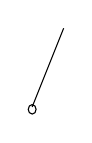
\begin{tikzpicture}[baseline=0cm,x=1cm,y=1cm]\draw[thin] (0,-.5)--(.4,.5);\draw[thin] (0,-.53) ellipse (.05 and .06);\end{tikzpicture}}. - It would remain finally to determine the effectivity structure in the category $\mathrm{Fcriso}(k)$ de\deleted{\unsure{termined}}\handwritten{\unsure{termined}} by the preceding recipe\deleted{\unsure{.} the natural suggestion is that $\mathrm{Fcriso}^{\handwritten{+}}(k)$ is generated by the images of $\mathrm{Fcriso}^{\handwritten{+}}$} Now it is immediate that the effectivity of an F-isoc\unsure{\.{r}|r}\unsure{\.{r}|y}stal is invariant under base change, in particular under the base change $k\handwritten{\longrightarrow\bar{k}}$, which reduces to the case of an algebraically closed $k$, or again to the case of $\underline{F}_p$ . \deleted{In}\handwritten{In} \deleted{terms of} the terminology introduced below, one will therefore find that the effective $\unsure{\mathbb{F}|\rlap{$G$}F|F|E}$-isocrystals are those which are \uline{of slope} $\handwritten{\geq}0$ (i.e. all of whose nonzero isoclinic components \deleted{are} are of slope $\handwritten{>}\ 0$).

\handwritten{8.} It therefore remains to study the gerbe $\underline{G}(\underline{F}_p)$, with it\unsure{\rlap{s}s|s|s}\deleted{n} \deleted{fiber functor,} canonical section over $\underline{Q}_p$, its extension structure, and its effectivity structure.

\margin{\handwritten{\figure{\begin{tikzpicture}\draw (0,0) -- (0.65,0.04) -- (0.65,0.8) -- (1.1,0.8);\end{tikzpicture}}}}
\inserted{\handwritten{8.1.}}\handwritten{\begin{tikzpicture}[baseline=0cm,x=1cm,y=1cm]\draw[gray,thin] (0,-.35)..controls (-.13,-.1) and (.05,.04)..(.1,.1)--(.8,.08)..controls (1,.08) and (1.1,.15)..(1.08,.25);\end{tikzpicture}} First of all, the datum of the canonical fibre functor allows one to identify $\underline{G}(\underline{F}_p)$ with the trivial gerbe\handwritten{\begin{tikzpicture}[baseline=0cm,x=1cm,y=1cm]\draw[gray,thin] (0,-.35)--(.27,.45);\end{tikzpicture}} defined by the band \inserted{\handwritten{$G$}}\handwritten{\begin{tikzpicture}[baseline=0cm,x=1cm,y=1cm]\draw[gray,thin] (0,-.35)--(.27,.45);\end{tikzpicture}} of this gerbe. As $\mathrm{Fcriso}(F_p)$ with its fibre functor is identified with the category of automorphisms of\inserted{$F_E$}\handwritten{\begin{tikzpicture}[baseline=0cm,x=1cm,y=1cm]\draw[gray,thin] (0,-.35)--(.27,.45);\end{tikzpicture}} finite-dimensional vector spaces\inserted{$E$}\handwritten{\begin{tikzpicture}[baseline=0cm,x=1cm,y=1cm]\draw[gray,thin] (0,-.35)--(.27,.45);\end{tikzpicture}} over $\underline{Q}_p$, with the functor ``forgetting $F_E$ '', one sees that the band of the gerbe is the $\underline{Q}_p$-\inserted{pro}\handwritten{\begin{tikzpicture}[baseline=0cm,x=1cm,y=1cm]\draw[gray,thin] (0,-.3)..controls (-.08,-.12) and (.13,.1)..(.25,.08)..controls (.65,.01) and (1,.14)..(1.12,.45);\end{tikzpicture}}algebraic envelope of the discrete group $\underline{Z}$ . Let $G$ be this affine group over $\underline{Q}_p$ . It\begin{tikzpicture}[baseline=(l.base),x=1cm,y=1cm]\node[inner sep=0pt] (l) {l};\draw[thin] (-.17,.55)--(.13,.55)--(.13,.62);\draw[thin] (-.05,.55)--(-.05,.61);\draw[thin] (-.17,-.12)..controls (.06,-.07) and (.04,-.13)..(.01,-.4);\end{tikzpicture} is evidently commutative, hence a product of a vector group $G_u$ with a group of multiplicative type $G_{\deleted{\unsure{m}}r}$ .
\margin{\handwritten{\unsure{reference|cf}\figure{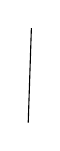
\begin{tikzpicture}\draw (0,0) -- (0.04,1.2);\end{tikzpicture}}}}
The latter is the multiplicati\deleted{ve}\handwritten{ve}\inserted{-type}\handwritten{\begin{tikzpicture}[baseline=0cm,x=1cm,y=1cm]\draw[gray,thin] (0,-.2)..controls (0,.08) and (.27,.06)..(.4,.07)--(1.6,.1)..controls (1.8,.12) and (1.8,.13)..(1.74,.33);\end{tikzpicture}} envelope of the group $\underline{Z}$, and it follows at once that it is the group of multiplicative type whose character group over $\handwritten{\bar{\underline{Q}}}_p$ is given by
\[
\handwritten{\Gamma}=\handwritten{\bar{\underline{Q}}}_p^{\handwritten{*}}\ ,
\]
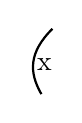
\begin{tikzpicture}[baseline=(x.base),x=1cm,y=1cm]\node[inner sep=0pt] (x) {\unsure{x}};\draw[thick] (.1,.45)..controls (-.2,.15) and (-.2,-.1)..(-.04,-.38);\end{tikzpicture}isomorph\unsure{\rlap{o}i|i|o}sm compatible with the action of $\operatorname{Gal}(\handwritten{\bar{\underline{Q}}}_p/\underline{Q}_p)$ ). On the other
